\documentclass[12pt]{article}

%% - - - page formatting
% \renewcommand{\baselinestretch}{2.0}
\usepackage[doublespacing]{setspace}
\usepackage[margin=1in, left=1in, top = 1in, includefoot, a4paper]{geometry} 
\usepackage[document]{ragged2e}
\setlength{\RaggedRightParindent}{2em}
\RaggedRight
\usepackage{indentfirst}
\setlength\footnotemargin{0em}
\usepackage{appendix}

%% - - - Citations & References
\usepackage[style=apa]{biblatex}
\addbibresource{./references.bib}

\usepackage{hyperref}
\hypersetup{
    colorlinks = true,
    urlcolor = blue,
    citecolor = [rgb]{0, .121, .388},
    linkcolor = [rgb]{.349, 0, 0},
}

% personal preference :)
\let\oldcite=\cite
\let\oldtextcite=\textcite
\renewcommand{\cite}[1]{\textcolor[rgb]{0, .121, .388}{\oldcite{#1}}}
\renewcommand{\textcite}[1]{\textcolor[rgb]{0, .121, .388}{\oldtextcite{#1}}}


%% - - -  Math
\usepackage{mathtools}
\usepackage{algorithm}
\usepackage{algorithmic}

%% - - - Media
\usepackage{graphicx}
\usepackage[rightcaption]{sidecap}

\pagenumbering{roman}



\title{Graphs as a Fundamental Data Structure in Human Cognition}
\author{Matt Wetzel}


\begin{document}

% % % % % % % % % %
%
%   TITLE
%
% % % % % % % % % %
\maketitle
\pagebreak

\tableofcontents
\pagebreak






% - - - - - - - - - - - - - - - - - - - - - - - - - - - - - - - - - - - - - - - - - - - - - - - - - - - - - - - - - - - - - - - - - - - - - - - - - - - - - - - - - - - - - - - - - - - - - - - - - - - - - - - - - - - -





% % % % % % % % % %
%
%   CONTENT
%
% % % % % % % % % %

\section{Introduction}
\pagenumbering{arabic}

The ability to generalize knowledge about the objects and events we've experienced to the objects and events we've yet to experience is a fundamentally important aspect of human cognition. This ability is likely mediated (in part) by our capacity to group objects and events into categories for later classification and inference. A great deal of the research on human category learning has typically relied on sequential presentation of stimuli (sampled from an experimenter-defined set), often defined by very few, easily identifiable features (\cite{kurtz2015human}). This paradigm is particularly useful for testing computational theories of cognition (\cite{wills2012adequacy}), given that the simple, abstract stimuli leveraged by category learning researchers can be represented as feature vectors (a data structure that's easy to integrate into computational algorithms). However, featural information is not the only information available to learners when making classification and inference decisions. How features, stimuli, and categories relate to each other can be very useful for human learners. If computational theories of categorization aim to elucidate the role of relational information during classification and inference, then they may benefit from a type of data structure that explicitly captures relations.

\subsection{Graph Theory \& Applications}

A graph is a type of data structure defined by a set of \textbf{nodes} and \textbf{edges} (\cite{newman2003structure}). A node can represent any kind of object or concept, while an edge represents some way in which 2 nodes are related. An edge can represent either a one-way connection from one node to another (\textbf{directed edge}), or a bidirectional connection between 2 nodes (\textbf{undirected edge})\footnote{ The directionality of an edge or graph depends on the type of system being represented.}. The \textbf{degree} of a node is defined by its number of edges. The \textbf{neighborhood} of a given node is the set of nodes it connects to. A set of nodes that all share a connection is referred to as a \textbf{clique}. The \textbf{distance} between two nodes is the number of edges that spans the path that connects them. The \textbf{density} of a graph typically describes total number of existing edges\footnote{ While this terminology paragraph might seem arbitrary, the types of reasoning that can be performed on a graph are often constrained by these various properties. If humans perceive and represent their environment as graphs, then this terminology should be useful for describing human reasoning as well}. Graph structured reasoning typically encompasses utilizing these properties of graphs to accomplish a few key objectives: inference \& classification of \emph{nodes}, inference \& classification of \emph{edges\footnote{ commonly referred to as \emph{link completion}}}, and inference, classification, \& generation of entire \emph{graphs} (\cite{wu2020comprehensive}). 

% FIGURE: Basic Graph 
\begin{SCfigure}[0.5][h]
    \centering
    \label{fig:basicGraph}
    \caption[basic graph]{a visual representation of a basic graph with numbered nodes and undirected edges (image taken directly from: \href{http://en.wikipedia.org/wiki/Graph_theory}{\emph{wikipedia}}).}
    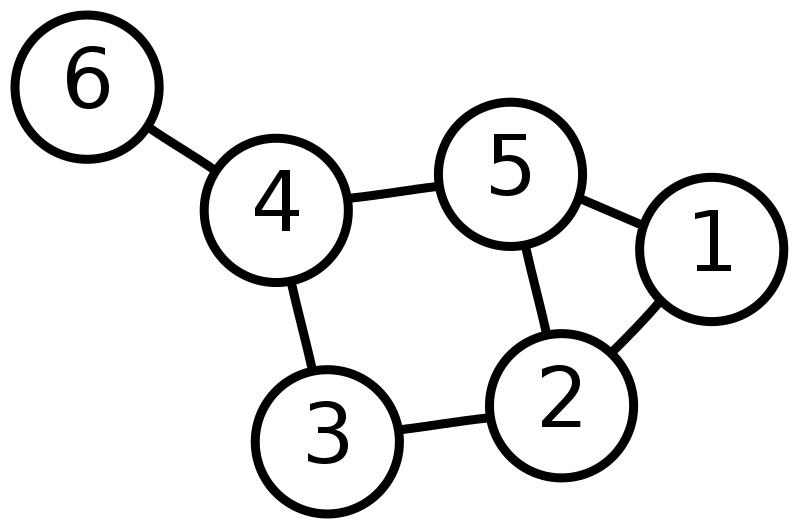
\includegraphics[width=.6\textwidth]{figures/basicGraph.png}
\end{SCfigure} 

Graphs have been used to describe and study a large variety of real world systems. For example, representing the Internet as a collection of websites (nodes) and links (edges) is foundational to modern search engines (\cite{newman2003structure}). A fundamental, century-old doctrine of neuroscience describes information processing in the brain as a directed graph of neurons connected via synapses (\cite{bullock2005neuron}). Graphs are a key data structure used to describe communities of users on social media platforms, where individuals are represented as nodes and their associations/communications are represented as edges (\cite{arya2018exploiting}). Additionally, scientific publications can be represented as a graph where papers (nodes) connect to other publications via citations (edges). Given the vast number of structured learning domains that exist, reasoning and statistical analysis of graphs has recently seen a surge of interest in the engineering and machine learning community (\cite{bronstein2017geometric}).

Despite the ubiquitousness of graphs in the natural world, reasoning on graphs is inherently difficult. Unlike sensory data (e.g., sight, sound) or symbolic descriptions (e.g., hand-coded feature vectors), graphical data has no guaranteed, consistent structure that can be exploited for computation (\cite{bronstein2017geometric,wu2020comprehensive}). However, the structural variability of graphs that make reasoning difficult are the very thing that make them powerful for learning and inference. For example, if I wanted to make inferences about an individual, I can leverage knowledge about that individual's friends and associates without knowing anything about the individual at all. Across many domains, the structural properties of graphs provide a powerful source of information for learning within a given domain, and even across unlearned domains as well (\cite{graves2016hybrid}).

\subsection{Core Argument of This Paper}

\emph{\textbf{Premise 1:}} It's intuitively reasonable to assume that some of the objectives of a category learning system are to correctly classify and infer the properties of objects and events (\cite{markman2003category}). Computational models of category learning typically accomplish these goals by learning some mapping between exemplars of a category and category labels, typically via exposure to one isolated item at a time (\cite{nosofsky2011generalized,kruschke1992alcove,kurtz2015human,love2004sustain}).

\emph{\textbf{Premise 2:}} Critically, machine learning researchers and engineers have highlighted that many real world systems can be described as a graph of interconnected objects and relations. Importantly, the qualitative and statistical properties that describe graphs provide a powerful medium for classification and inference regarding objects and their relationships, as well as the construction of entire graphs themselves (\cite{schlichtkrull2018modeling,bronstein2017geometric}). 

\emph{\textbf{Argument:}} If the objectives of category learning are classification and inference in real world domains, and graphical representations provide a powerful medium for those objectives, then it's relatively straightforward to speculate that humans leverage graph structured representations for category learning. If so, it would be reasonable to assume that \textbf{(a)} humans might be sensitive to the various  properties of graph structured learning domains, and \textbf{(b)} cognitive representations might be structured graphically themselves. The first section of this paper will highlight key research across different branches of psychology that address whether either of those assumptions are plausible. Then, the implications of graphical representations on two critical phenomena within the category learning literature (similarity \& unidimensional bias) will be discussed. Finally, this paper will explore the argument that many aspects of cognition can be framed as computational operations on graph structured representations. 

% - - - - - - - - - - - - - - - - - - - - - 

\subsection{Are Humans Sensitive to Graph Structured Learning Domains?}

Language learning has been a very rich testing ground for testing humans' sensitivity to graph structured learning problems, typically referred to as \emph{Network Science} (\cite{lynn2019graph}). Network science has provided an explanatory framework for human language at many different levels, including language acquisition via statistical learning (\cite{saffran1996statistical,lynn2019graph}), word recognition \& the mental lexicon (\cite{vitevitch2008can,chan2009influence}), and speech production (\cite{chan2010network}). Language and speech provide a particularly interesting network structure: both the syllables within words and words within sentences\footnote{and even the ideas and topics that words convey} are constrained by a probabilistic, temporal order. The temporal relationship shared by the discrete units of language can be represented as a graph of transition probabilities.

In a foundational study that laid the groundwork for the utilization of network science in language, \textcite{saffran1996word} demonstrated that young adults were sensitive to the transition probabilities between phonemes in a made-up language. With the goal of studying the mechanisms of sound segmentation in language, \textcite{saffran1996word} exposed subjects long audio streams of unsegmented speech sounds that utilized 12 unique syllables clustered to form 6 unique 3-syllable words. Because the audio stream was unsegmented, there were no pauses to indicate when one word stops or another began. Critically, the probability that one syllable would transition from another were embedded in the 6 words used in the audio stream, such that within-word syllable transitions were more likely than between-word syllable transitions. At test, subjects decided which of two possible word choices belonged to the made-up language. The key finding was that subjects were able to recognize the original words from the language when compared to words with 3-syllable combinations that were statistically unlikely (i.e., ``nonword'' foils with average syllable transition probabilities of 0). In addition, subjects could even recognize the difference between original words and pseudo-word foils (where only one syllable transition was statistically unlikely), albeit with worse performance relative to nonwords. Even further, \textcite{saffran1996statistical} replicated this phenomena in 8-month old infants (using a novelty-preference paradigm for assessing sensitivity to statistically likely or unlikely syllable combinations)\footnote{ Under the assumption that infants spend longer time listening to novel stimuli, \textcite{saffran1996statistical} found that infants spent more time ``listening'' to nonwords than real words in the made-up language}.

Saffran \& colleagues' work demonstrated that humans are sensitive to the transition probabilities of syllables in language, hypothesizing that humans can leverage these statistics (among other cues) to segment otherwise continuous speech signals into discrete linguistic units (e.g., words)\footnote{the ability to segment information from a continuous medium into discrete signals might also relate more generally to human categorization as well}. Similar findings have been extended with visual presentation of shapes and scenes as well (\cite{turk2005automaticity,brady2008statistical}). While the notable result from these demonstrations is that humans leverage transition probabilities during learning, the serial presentation paradigm itself has a very interesting property: the collective body of stimuli and their transitions form the basis of a graph. Interestingly, a host of recent findings suggest that humans are not only sensitive to transition probabilities of stimulus presentations, but also sensitive the structural properties of transition graphs as well (\cite{lynn2019graph,kahn2018network,karuza2017process,karuza2019human}). 

\textcite{kahn2018network} provide a notable demonstration of humans' sensitivity to the structure of transition graphs. In their experiments, subjects were instructed to press sequences of keys on a keyboard. The task was self-paced, and subjects were given a signal on each trial regarding which key to press next. The probability of one key transitioning to another was defined by a particularly structured graph representing keys as nodes and transitions as edges. Critically, subjects were trained on 3 different types of graphs: a modular graph\footnote{ Interestingly, many natural graphs in the real world have a modular structure (\cite{kahn2018network}).}, a lattice\footnote{ A \href{https://en.wikipedia.org/wiki/Lattice_graph}{lattice} is a structured graph with no modularity.}, and a random graph with no modularity or structure. One critical finding was that the modular graph was much easier to learn than the lattice or random graphs (which themselves did not differ in learnability). Additionally, \textcite{kahn2018network} found that subjects' reaction times were much slower when crossing edges between modules\footnote{or, densely connected clusters} in the modular graph structure (referred to as a \emph{cross-cluster surprise effect}). This is interesting given that each edge had an equally likely transition probability; \textcite{kahn2018network} attribute these distinctly slower reaction times as evidence of subjects' sensitivity to higher-order structure in the transition graph.

\begin{figure}[h]
    \centering
    \label{fig:kahn2018network-figures}
    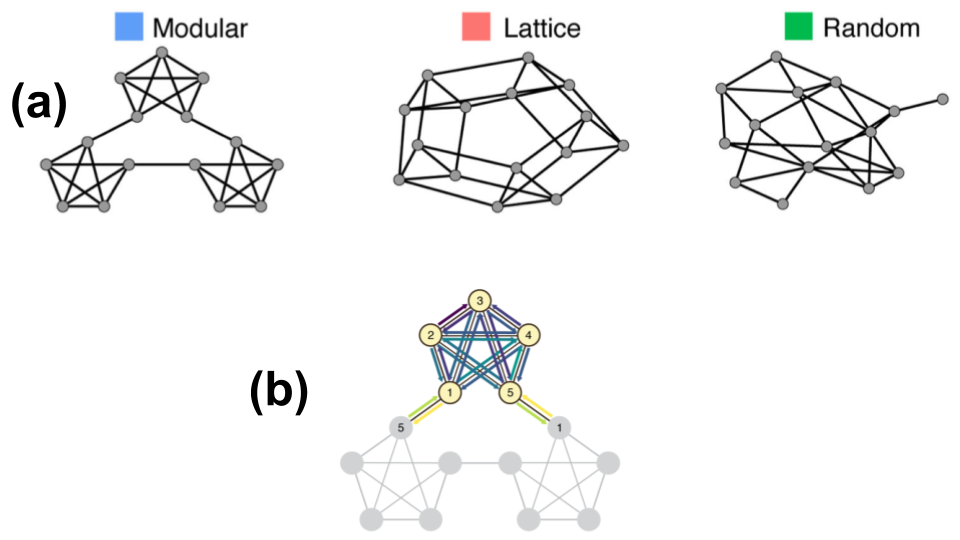
\includegraphics[scale=.4]{figures/kahn2018network-figures.png}
    \caption[Kahn et al., 2018]{\textbf{(a)} Graph structures used in \textcite{kahn2018network}. Note the three distinct clusters in the modular graph. \textbf{(b)} Reaction times for different key transitions (edges) in the modular graph (yellow indicating longer RTs). Taken directly from \emph{\textcite{kahn2018network}}.}
\end{figure} 

In a similar demonstration, \textcite{karuza2019human} found slower reaction times at cross-cluster boundaries across different graphs that varied in their community structure. Subjects were shown sequences of visual stimuli\footnote{ The stimuli used were images of realistic looking 3D objects that were difficult to identify (\cite{horst2016novel}).}, and asked to identify whether each stimulus was presented at it's normal orientation (which was established via a prior training phase). Importantly, the order of stimulus presentation was defined by the graph representing each visual stimulus as a node and the transition to a new stimulus as an edge. \textcite{karuza2019human} replicated the cross-cluster surprisal effect in a variety of graphs with different numbers of local communities\footnote{ ranging from 2-6 communities each}. This work highlights that humans are sensitive to boundary conditions in a variety of graph structured learning problems, across multiple cognitive domains. In a similar preparation, \textcite{karuza2017process} found that the particular \emph{path} used to sample nodes and their transitions mediated subjects' sensitivity to cluster boundaries, clarifying that subjects knowledge of network structure reflects the way in which the network is traversed. 

These demonstrations are compelling evidence that humans are sensitive to both local and global properties of network structured learning domains. However, these preparations all utilize a very particular type of experimenter-defined graph where edges are defined by stimulus transitions (\cite{kahn2018network,karuza2017process,karuza2019human}). More evidence is needed to support whether humans are sensitive to complex learning domains in nature, where the number of nodes and edges are vast and the structural statistics are very complex. Phonological relationships between English words provide an interesting real-world domain that has been leveraged to explore humans' sensitivity to highly complex networks in nature (\cite{vitevitch2008can,vitevitch2012complex,chan2009influence,chan2010network}).

An average English-speaking adult is estimated to have an awareness of around 17,000 words (\cite{goulden1990large}). In a recent analysis, \textcite{vitevitch2008can} attempted to elucidate the undirected graphical structure that describes the phonological similarity between words\footnote{A given word is \emph{phonological neighbor} to another word if it can subsume the form of that word by the addition or removal of a single phoneme; phonological similarity has been implicated in a number of phenomena in the language learning literature (\cite{vitevitch2008can})}. In addition to other descriptive network statistics like average path length and degree distribution\footnote{i.e., average neighborhood size of each node}, \textcite{vitevitch2008can} identified that the global \emph{clustering coefficient} of the phonological graph of English words is much higher than what would be expected from a randomly connected graph. The global \emph{clustering coefficient} describes the degree to which a typical node's neighbors are also connected to each other\footnote{Interestingly, graphs with a high clustering coefficient are empirically easier to navigate (\cite{porter2012small}), and have many other useful properties (\cite{vitevitch2008can})}. 

Critically, the clustering coefficient of a single node has a meaningful influence on lexical processing. \textcite{chan2009influence} found that vocally-presented words with a low clustering coefficient were much easier to identify through background noise than words with a high clustering coefficient\footnote{\textcite{chan2009influence} hypothesize that this confusability might arise from within-cluster interference during the spreading-activation of representations in the mental lexicon}. Utilizing a picture-naming task, \textcite{chan2010network} found that subjects took longer to produce words with high clustering coefficients. Additionally, \textcite{chan2010network} reanalyzed data from a prior study of speech errors (\cite{fay1977malapropisms}) and found that errors were more likely to occur for words with high clustering coefficients. Even further, \textcite{vitevitch2012complex} found that words with high clustering coefficients were more accurately remembered in a recognition task, and led to higher false-alarm rates in a false-memory task. Together, these results suggest that phonological network structure of the English language has important consequences on speech recognition, speech production, and memory.

\begin{figure}[h]
    \centering
    \label{fig:chan2010network-figure}
    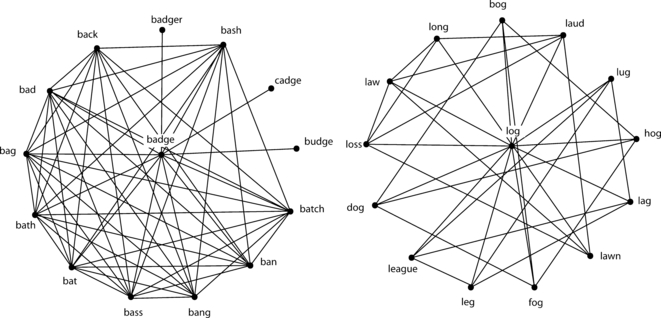
\includegraphics[scale=.6]{figures/chan2010network-figure.png}
    \caption{Comparison of the neighborhood structure of a word with a high clustering coefficient (left) and a low clustering coefficient (right); Taken directly from \emph{\textcite{chan2010network}}.}
\end{figure} 

While there is an increasing amount of evidence that humans are sensitive to the network structure present in various learning domains (\cite{saffran1996word,karuza2019human,karuza2017process,kahn2018network,vitevitch2012complex,chan2009influence,chan2010network}), these studies alone don't directly address whether cognitive representations embody network structures themselves (though they are certainly suggestive). The next section will explore the psychological plausibility that cognitive representations leverage graphical structure.

% - - - - - - - - - - - - - - - - - - - - - 

\subsection{Are Graphical Representations Psychologically Plausible?}

The idea that cognitive representations leverage graphical structure dates back to the well-known \emph{spreading activation} theory (\cite{collins1969retrieval,collins1975spreading}). Building off of \textcite{quillian1967word}'s symbolic framework of representing semantic meaning and inheritance in computers, \textcite{collins1969retrieval} proposed that human semantic memory is structured as a conceptual hierarchy\footnote{Note that a hierarchy is a type of acyclic graph known as a \emph{tree}}, where superordinate categories branch into subordinate categories (see figure \ref{fig:spreading-activation}). In their seminal demonstration, \textcite{collins1969retrieval} had subjects determine the truthfulness of certain assertions about the properties of objects/concepts; the properties of each assertion were relevant to different ``levels'' of the conceptual hierarchy. Importantly, the path distance between the target object and its given property was predictive of the speed at which subjects responded.\footnote{For example, two sentences might be: ``A canary is an animal'' or ``A canary is a bird''. Subjects should respond faster to the former sentence, since the property \emph{bird} is closer to \emph{canary} along the conceptual hierarchy than \emph{animal}.}. \textcite{collins1969retrieval} took this as evidence that human semantic memory is represented as a hierarchical graph\footnote{This assumption was later relaxed in \textcite{collins1975spreading}} (or, a tree).

\begin{figure}[h]
    \centering
    \label{fig:spreading-activation}
    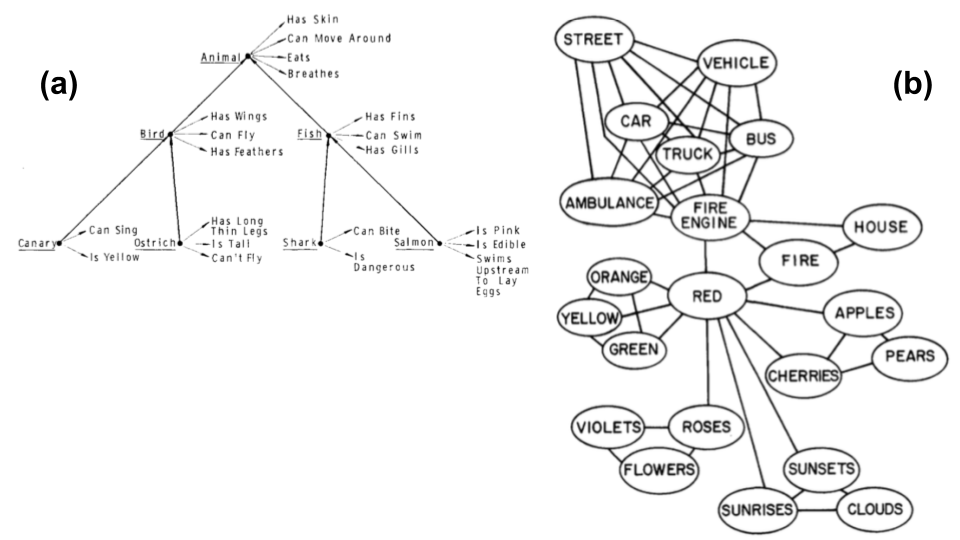
\includegraphics[scale=.4]{figures/spreading-activation.png}
    \caption{\textbf{(a)} Conceptual hierarchical as a model of human semantic representations proposed by \textcite{collins1969retrieval}. \textbf{(b)} Extended version proposed by \textcite{collins1975spreading} that relaxes the hierarchical and acyclic assumptions. Taken directly from \emph{\textcite{collins1969retrieval} \& \textcite{collins1975spreading}}.}
\end{figure} 

While certainly compelling, \textcite{collins1969retrieval} demonstration lacks predictive value as a model of cognitive representations. Given that the structure of a semantic network can be modified to ``fit'' any set of experimental results, \emph{spreading-activation theory} lacked falsifiability (\cite{o2009conceptual}). In an interesting demonstration, \textcite{steyvers2005large} help resolve this lack of falsifiability by tethering the hypothetical structure of semantic networks to a large corpus of word association norms from \textcite{nelson2004university}\footnote{In \textcite{nelson2004university}, around 149 students were shown a word, and asked to provide the first associated word that they thought of in response.}. \textcite{steyvers2005large} performed a network analysis on the graph of word association norms, where each word (node) is connected according to the likelihood that it will trigger another word in a free association task. \textcite{steyvers2005large} found that the graph of word association norms embody a similar structure to many graphs in nature (including the phonological similarity network analyzed by \cite{vitevitch2008can}), and laid the groundwork for integrating corpus analysis into the study of human semantic processing. In similar work, \cite{abbott2012human} found that the results of a free association task could be predicted by a random walk algorithm on along a semantic network\footnote{Interestingly, \textcite{griffiths2007google} found that Google's Page Rank algorithm for navigating the Web could also be leveraged to explain free association data in humans.}. 

The findings that graph traversal algorithms can explain human semantic associations is promising evidence that cognitive representations leverage graphical structure (\cite{steyvers2005large,abbott2012human,griffiths2007google}). However, independent of what cognitive representations actually are, an important constraint for any model of representations is that it be feasible to implement using neural hardware. Are graphical cognitive representations neurologically plausible? Though individual networks of neurons in the brain are an example of a graphical system (\cite{newman2003structure,bullock2005neuron}), whether neural activity manifests as graphical cognitive representations is an open question. However, a number of studies using a variety of neurophysiological methodologies have begun to explore this question (\cite{garvert2017map,schapiro2013neural,bassett2010efficient}).

Representational similarity analysis (RSA; \cite{kriegeskorte2008representational}) is a methodological framework for exploring cognitive representations via the pairwise similarity of objects / stimuli on some psychological or physiological metric (e.g., similarity ratings or fMRI activity). A basic assumption of RSA is that the representation of two objects are similar if they elicit a similar measurement on some metric of choice. Leveraging this basic assumption, \textcite{garvert2017map} had subjects sequentially view images of objects while recording brain activity via fMRI. The order in which stimuli were selected was based on a random walk through a transition graph (similar to \cite{karuza2019human,kahn2018network}). \textcite{garvert2017map} found that the pairwise similarity between objects activations in of the entorhinal cortex (a mediator in the hippocampal memory system; \cite{witter2011entorhinal}) was predicted by the path length between objects in the transition graph. In a similar preparation, \textcite{schapiro2013neural} found that community structure in a modular graph was also predictive of pairwise representational similarity in the Inferior Frontal Gyrus, the Anterior Temporal Lobe, and Superior Temporal Gyrus (using the same modular graph from \cite{kahn2018network}). Interestingly, each of those brain regions is implicated in processing semantic meaning (\cite{schapiro2013neural}). In a more macro-level analysis of brain functioning, \textcite{bassett2010efficient} found evidence of modularity in the graph representing the covariability in bold responses of various brain regions.

Graphical models provide an efficient way of storing the relatively massive amount of semantic and conceptual knowledge that humans possess (\cite{collins1969retrieval,abbott2012human}); in addition, a number of studies highlight the plausibility of graphical representations in human cognition (\cite{steyvers2005large,garvert2017map,bassett2010efficient}) and that humans are sensitive to the network structure of various learning domains (\cite{karuza2017process,kahn2018network,karuza2019human,chan2009influence,chan2010network,vitevitch2012complex}). Given the productiveness of applying graph theory and network science to the study of human language and semantic processing, the next section will highlight relatively unaddressed implications of graphical representations on human category learning.

% - - - - - - - - - - - - - - - - - - - - - 

\section{Implications of Graphical Representations on Category Learning}

Graph structured representations have an interesting history in the category learning literature (going beyond \textcite{collins1969retrieval}'s assertion of a graphical representation of semantic meaning and category hierarchies). Early theorists recognized the importance of hierarchies in natural categories (\cite{collins1969retrieval,mervis1981categorization,palmeri1999learning}; though see \cite{sloman1998categorical}), which embody a very particular type of graphical structure (a tree). Additionally, many leading models of category learning are instantiated as a graph using the connectionist framework\footnote{Connectionist models are a particular class of graphical models that leverage distributed representations (\cite{mcclelland1987parallel,griffiths2010probabilistic})} of cognition (\cite{kurtz2007divergent,kruschke1992alcove,rogers2004semantic}). Even the classic exemplar (\cite{nosofsky2011generalized}) and prototype (\cite{minda2001prototypes}) theories of category learning can be interpreted as directed graphical models mapping features to probability distributions (\cite{danks2007theory}). Despite many theories independently invoking the idea that category representations are graphical in nature, there is very little work connecting category learning and network science. The next section will explore whether the language of network science can address any fundamental, ongoing issues in the category learning literature.

\subsection{Unidimensional Bias as \emph{Small World} Regularization}

Traditional, artificial classification learning (TACL) has been a widely used paradigm for studying human category learning in the lab (\cite{,kurtz2015human,nosofsky1994comparing,markman2003category}). TACL experiments typically involve repetitively exposing subjects to visual stimuli (one at a time); on each trial, subjects guess the category label of the presented stimulus (given a set of options). The category labels of the stimuli are predefined by the experimenter, often specified in a way that helps disentangle different theoretical accounts. Stimuli are often composed of very simple objects with highly identifiable features, which can easily be represented as a feature vector of discrete or continuous values. The TACL paradigm has been a very productive avenue for advancing computational theories of category learning, uncovering a number of important phenomena that have become theoretical benchmarks in the modeling endeavor (\cite{kurtz2015human,wills2012adequacy,nosofsky1994comparing}).

One notable benchmark phenomenon is the unidimensional bias; that is, the well-replicated finding that humans are especially adept at learning categories defined by a single feature (\cite{shepard1961learning,nosofsky2011generalized,kruschke1993human}). In addition, when asked to freely sort a set of objects into separate categories, humans tend to prefer sorting categories on the basis of single feature (\cite{medin1987family,,ahn1992two,ashby1995categorization,milton2009neural}). In a foundational study, \textcite{medin1987family} gave subjects an array of stimuli and asked them to sort the stimuli into 2 equal groups. The stimuli varied according to 5 relevant, binary features (that could take on 2 possible values/states). Importantly, the stimuli were selected by the experimenters from a 2-category structure defined by \emph{family resemblance}, where each stimulus has most features in common with one of 2 \emph{prototypes}\footnote{The \emph{Family Resemblance} category structure is notable in that it seems to underlie many categories in the natural world (\cite{rosch1975family})}. Across several experiments, subjects (who were unaware of the actual category structure that stimuli were sampled from) were much more likely to sort categories into groups based on a single dimension\footnote{In fact, some of \textcite{medin1987family}'s experiments failed to show any behavior besides unidimensional sorting}. 

Why might the unidimensional bias be theoretically unintuitive, despite consistent replication in the category learning literature? Many theorists have argued that a ``ideal'' category structure should group exemplars so that members of the same category are featurally similar, while members from opposing categories are featurally dissimilar (\cite{medin1987family,rosch1975family}). The \emph{family resemblance} structure is ideal in that it accomplishes that goal (in addition to being prevalent in natural categories). On the contrary, a unidimensional category does not \emph{seem} to consistently meet this optimization goal; it might produce exemplars that are identical on the basis of one feature, but would allow exemplars to be radically different when considering other features\footnote{For example, \emph{apple} and \emph{firetruck} both belong to the category of \emph{red objects}, but share very few features in common.}. Many successful accounts of category learning leverage selective attention as a mechanism to prioritize a unidimensional bias (\cite{nosofsky2011generalized,kruschke1992alcove,love2004sustain}); selective attention is likely a critical factor in why some theoretical accounts succeed relative to others.

There are various explanations as to why unidimensional bias might be so prevalent despite it's clash with historic theories about what defines an ``ideal'' category structure. Some researchers have argued that focusing on a single dimension requires less effort than integrating all features into a similarity computation (\cite{wills2013overall}). Another theoretical suggestion comes from \textcite{feldman2000minimization}, who demonstrated that a family resemblance category structure in the domain of binary-featured stimuli has a higher degree of \emph{boolean complexity} than a unidimensional category structure\footnote{\emph{Boolean complexity} can be defined as the shortest possible mapping between the set of binary features and a dichotomous category label that can be realized by a boolean circuit (\cite{feldman2000minimization}).}. Both of these accounts are compelling (and neither are mutually exclusive). However, the next section will propose another (also not mutually exclusive) explanation of why the unidimensional bias might persist in human cognition (using a well known phenomena in the network science literature).

\emph{Small World}\footnote{The term \emph{small world} is in reference to the fact that it's unintuitively easy to find a short, associative path connecting two human beings despite the fact that the entire social network defining human communication is incredibly vast and complex (\cite{newman2003structure}).} networks are formally defined as a type of sparsely connected graph where the average path distance between nodes grows less rapidly as the number of nodes in the network increases (\cite{porter2012small}). Importantly, small world networks have a number of interesting statistical properties that commonly describe many real world graphs in nature, such as:

\begin{itemize}
    \item the WorldWideWeb (\cite{newman2003structure}),
    \item the human brain (\cite{bassett2006small}\footnote{though see \textcite{hilgetag2016brain} and \textcite{papo2016beware} for limitations to the small world model of neuroanatomy},
    \item the graph representing phonological similarity of English words (\cite{vitevitch2008can}, as described earlier),
    \item semantic networks generated from free recall experiments (\cite{steyvers2005large,nelson2004university}).
\end{itemize} 

Small world networks can be characterized as being sparsely connected, with a relatively smaller number of densely connected nodes acting as ``hubs'' connecting the rest of the nodes in the network (\cite{steyvers2005large}). Another important feature of small world networks is that they are relatively easy to navigate, particularly when the navigator has limited access to anything beyond local information  (\cite{newman2003structure}). While it might seem like a stretch to say that this ``easy to navigate'' property has any implications to human cognition, recall that \textcite{abbott2012human} demonstrated that human free association appeared particularly similar to a random walk along a graph of semantic associations. 

How might small world networks relate to the unidimensional bias in category learning? In a category learning experiment, stimuli are defined by a set of features that are each predictive (or not predictive) of some category label. Many category learning models can be functionally described as building probability density functions mapping features to category labels (\cite{ashby1995categorization}), reducing the problem of category learning to feature-label association. If the goal of the human categorization system is to produce isolated mappings between features and labels, it seems surprising that subjects might prefer the ``less-than-deal'' unidimensional category structure. However, note that the features and labels used in category learning studies bear close resemblance to the conceptual ``nodes'' researchers invoke when describing graphical models of human semantic representations (\cite{collins1969retrieval,collins1975spreading,love2004sustain}; see figure \ref{fig:spreading-activation}). If the goal of a categorization system is to construct and refine the complex semantic networks historically invoked by cognitive scientists (\cite{collins1969retrieval,collins1975spreading,sloman1998categorical,love1995mutability,steyvers2005large,abbott2012human}), then a unidimensional ``bias'' might serve a very functional purpose: regularizing sparsity in a graphical representation of our environment.

\textcite{steyvers2005large} found that the semantic network describing free association norms resembled a small world network, which are characterized as being sparsely connected. This sparse connectivity might make navigation through semantic networks more efficient (\cite{newman2003structure,abbott2012human}). How might a unidimensional bias enforce sparsity? \textcite{steyvers2005large} developed a recursive algorithm for generating the types of small world networks commonly found in nature. The algorithm starts with an initial set of fully connected nodes, incrementally adding new nodes with \(M\) connections to a randomly sampled neighborhood\footnote{\(M\) will influence how sparse the final network is}. \textcite{steyvers2005large} found that a relatively low \(M\) (of 11) can produce relatively large networks\footnote{5018 nodes in total} that retain some of the key elements of small world networks. 

Each iteration of the \textcite{steyvers2005large} algorithm seems intuitively analogous to the structure of a typical category learning experiment: one node (a category label) is probabilistically associated with a neighborhood of other nodes (the set of critical features present in each stimulus). If the mechanisms of category learning we typically isolate in the laboratory reflect some generative process of building a probabilistic network of knowledge about things and their features, then a unidimensional prior on probabilistic associations might lead to more efficient knowledge retrieval later on. As a proof-of-concept, large networks (with 200 nodes) were generated using the network building algorithm of \textcite{steyvers2005large}; the \(M\) parameter was adjusted for each. The result of this simulation highlight that the denser networks produced node degree distributions that deviate from what's expected in a small world network (figure \ref{fig:small_world_simulation}). While a unidimensional prior might be less-than-ideal in an isolated laboratory experiment, it might be a necessary trade-off for efficient navigation in representational space\footnote{Speculatively, reduction in graph density through the unidimensional bias may also lead to conceptual representations with less boolean complexity as well (\cite{feldman2000minimization}).}.

% show plot and double check results
% \pagebreak
\begin{figure}[p]
    \centering
    \label{fig:small_world_simulation}
    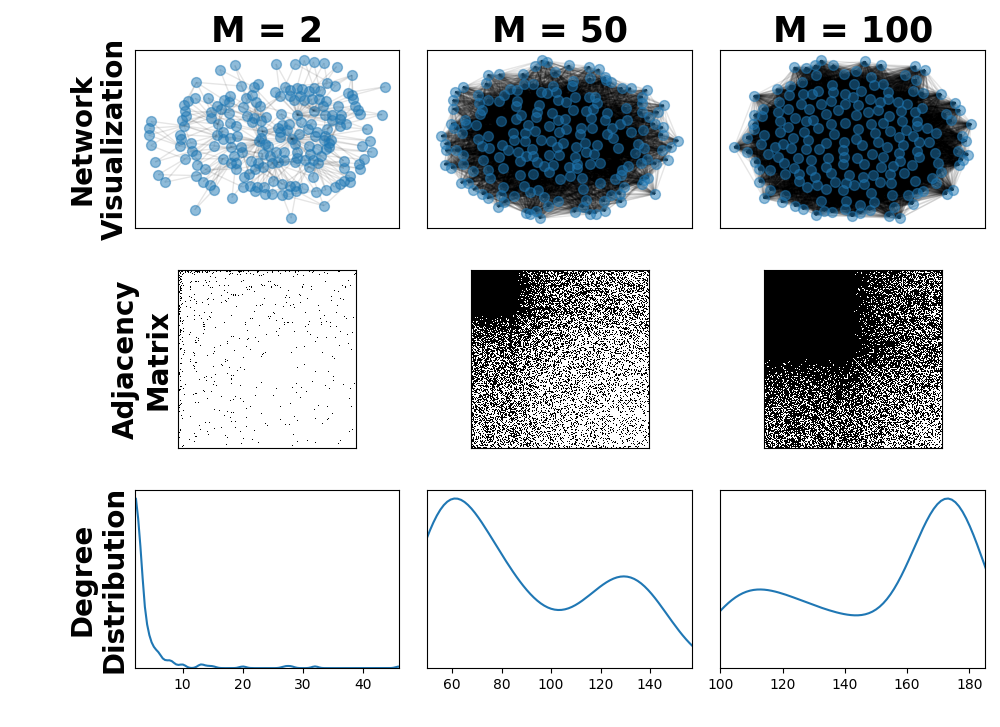
\includegraphics[scale=.6]{figures/small_world_simulation.png}
    \caption{Results from a simulation showing the network, adjacency matrix, and node degree distribution for 3 examples of a network built using the algorithm from \textcite{steyvers2005large}. Note that in all instances, the total number of nodes is held constant.}
\end{figure}


\subsection{Similarity, Graph Embeddings, and Path Length}

Similarity is a commonly invoked construct in many domains of cognition (\cite{goldstone1994role}), particularly for theories of categorization (\cite{shepard1987toward,nosofsky2011generalized,kurtz2015human,goldstone2012similarity}). An intuitive assumption about categories is that objects from the same category should be similar in some way. Many category learning models leverage a spatial interpretation of similarity, where the similarity between two stimuli (or between a stimulus and a category representation) is determined by their distance in some psychologically-transformed space (\cite{nosofsky2011generalized,kruschke1992alcove,minda2001prototypes}). While category learning models that rely on spatial similarity metrics have provided relatively successful accounts of human learning and generalization, spatial interpretations of similarity make a number of critical assumptions that violate numerous empirical findings (\cite{tversky1977features,tversky1982similarity,holyoak1983social,polk2002rating}. Additionally, similarity judgments in category learning models often only consider category representations and category exemplars in isolation, neglecting the impact of relational knowledge on similarity perception (\cite{goldstone1991relational,markman1993structural}).  The next section will contrast spatial and relational approaches to similarity, and highlight the strengths \& weaknesses of graphical representations for addressing unresolved issues in similarity research.

\textbf{\emph{Spatial Metaphor of Similarity}:} A widely prevalent (though controversial) assumption in psychology is that stimuli can be represented as vectors of values defined by their features (\cite{shepard1987toward,kurtz2015human})\footnote{For example, the representation of the squares in figure \ref{fig:spatialSimilarity} can be represented as a vector describing their size and shading}. There are number of phenomena that make this assumption seem viable. For example, \textcite{guttman1956discriminability} trained pigeons to produce pecking responses during the presentation of a color stimulus. After training, \textcite{guttman1956discriminability} varied the wavelength of the color stimulus and found that the frequency of pecking responses decreased monotonically as wavelength deviated from the value originally seen during training \footnote{The training wavelength in \textcite{guttman1956discriminability}'s experiment can be represented as a single point in a 1-dimensional, continuous space}. At a physiological level, the firing rates of individual neurons in the animal brain can be predicted by continuous functions mapping firing rates to stimulus dimensions (\cite{butts2006tuning,kang2004information}). \textcite{shepard1987toward} extended this idea by suggesting that the probability of stimulus generalization decreases exponentially as dissimilarity increases (i.e., a monotonic generalization gradient). Additionally, \textcite{shepard1987toward} relaxed any assumptions about true stimulus features and suggested that the exponential generalization gradient spanned some psychological space that could be inferred using a validated behavioral measurement (e.g., similarity ratings). 

\begin{figure}[h]
    \centering
    \label{fig:spatialSimilarity}
    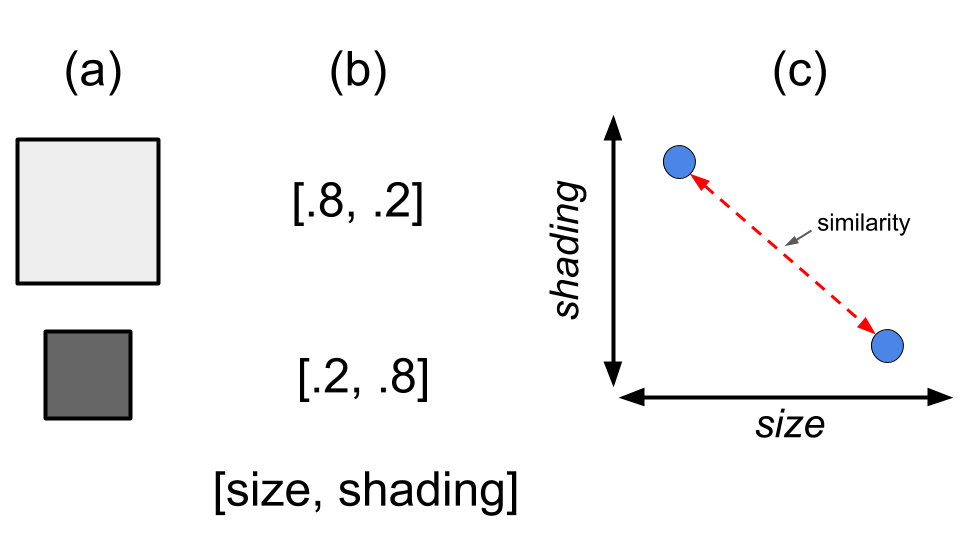
\includegraphics[scale=.4]{figures/spatialSimilarity.png}
    \caption{(a) Example of two stimuli, each with 2 core features (size \& shading). (b) Those same stimuli represented as feature vectors. (c) The two stimuli plotted in a continuous space.}
\end{figure}

The exponential decay function suggested by \textcite{shepard1987toward} has been leveraged by many successful models of human category learning, which typically utilize a similarity metric that compares the similarity of objects to some set of reference points. These \emph{reference points} might consist of previously experienced exemplars (\cite{nosofsky2011generalized,kruschke1992alcove}), category-specific centroids (\cite{minda2001prototypes,}), or category-independent centroids that capture densely populated areas of feature space (\cite{love2004sustain,rosseel2002mixture}). Critically, these models rely on stimulus descriptions that only consider stimulus features and associated category labels. This approach has been successful in adequately describing a number of empirical phenomena in the categorization literature (\cite{nosofsky1994comparing,kruschke1993human}). However, models leveraging similarity in feature space explicitly neglect any information about how exemplars and categories relate to each other or their given context. This shortcoming is critical given many empirical demonstrations that suggest an important role of relational knowledge in similarity perception (\cite{goldstone1991relational,markman1993structural,goldstone1994similarity}).

\textbf{\emph{Relational Knowledge and Similarity Perception}:} In category learning models described thus far, stimuli (or, exemplars) are defined by their \emph{features} (or, attributes). In an effort to highlight the dissociation between features and relations, \textcite{goldstone1991relational} asked subjects to pick which of 2 base stimuli was more similar to a target stimulus (figure \ref{fig:goldstone1991}). Critically, the base stimuli differed in the number of shared features or shared relations with the target stimulus. Across a series of experiments using a variety of stimulus sets, \textcite{goldstone1991relational} found that (a) subjects were more likely to choose the relationally similarity stimulus over the featurally similar stimulus, and (b) subjects choices were influenced by the number of existing relational or featural matches in the set. That is, subjects were more likely to choose the featurally similar stimulus when the number of pre-existing featural matches was high, and more likely to choose the relationally similar stimulus when the number of pre-existing featural matches was low. In addition to showing the role of relations in similarity perception, \textcite{goldstone1991relational}'s results suggest that the collective dynamics of features and relations impact similarity judgments in distinct ways.

\begin{figure}[h]
    \centering
    \label{fig:goldstone1991}
    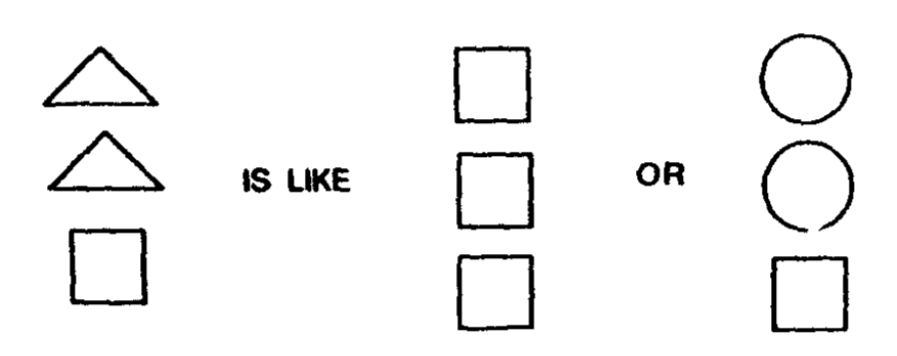
\includegraphics[scale=.4]{figures/goldstone1991.png}
    \caption{example of the task in \textcite{goldstone1991relational} (taken directly from \cite{goldstone1991relational})}
\end{figure}

In a different preparation, \textcite{markman1993structural} showed subjects pairs of scenes involving a set of related objects (figure \ref{fig:markman1993}). Subjects engaged in a \emph{one-shot mapping} tasks, where they were directed to find the item from the target scene that ``goes with'' the item from the base scene. Importantly, the target object was present in both scenes (though its relational role was different in each). If subjects were considering only the featural attributes of the scenes, then the obvious choice is to choose the same object as it appears in both scenes. However, \textcite{markman1993structural} found many instances where subjects mapped objects based on their relational roles in the scene (despite those objects having relatively dissimilar features). The likelihood for relational responding increased when subjects were asked to rate the similarity of the two scenes\footnote{on a scale from 1-9} before the one-shot mapping task. 

\begin{figure}[h]
    \centering
    \label{fig:markman1993}
    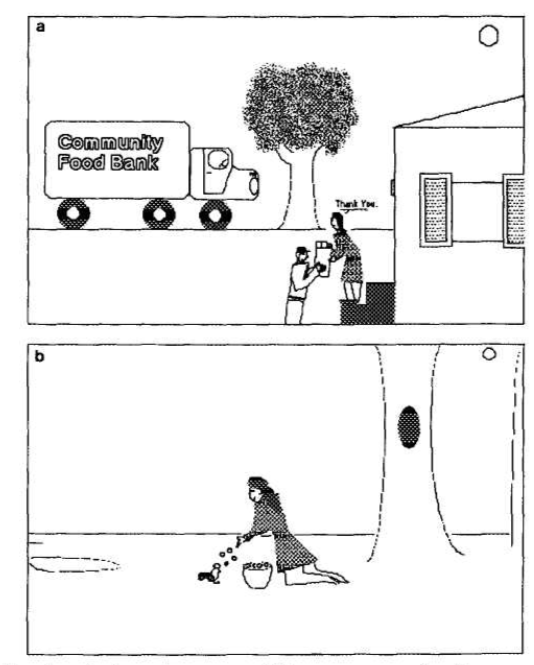
\includegraphics[scale=.6]{figures/markman1993.png}
    \caption{example of the stimulus preparation used in \textcite{markman1993structural} (taken directly from \cite{markman1993structural})}
\end{figure}


The importance of relational roles in similarity perception was explored further by \textcite{goldstone1994similarity}, who asked subjects to rate the similarity of two objects composed of features with identical roles (e.g., wings, tail, head, body). \textcite{goldstone1994similarity} found that similarity ratings were strongest when objects shared properties on features with the same role (e.g., both objects have red tails) than when the objects shared properties on features with different roles (e.g., object A has a red tail and object B has a red body)\footnote{The property used in this example (color:red) was not an actual property used by \textcite{goldstone1994similarity}}. These results highlight that the structural information defining a stimulus influences similarity perception in a way that's difficult to account for when stimuli are strictly represented as feature vectors in isolation. 

\textbf{\emph{Spatial Similarity and Graph Embeddings}:} In important question is whether findings from the relational similarity literature can be reconciled with findings that exponential distance is highly predictive of categorization and generalization behavior in human learners (\cite{shepard1987toward,nosofsky1994comparing,kruschke1992alcove,love2004sustain}). Typically, models leveraging spatial similarity computations treat stimuli as points in the space defined by their features (often modified using a multidimensional scaling algorithm that distorts the space to better reflect some other psychological property\footnote{for example, pairwise similarity ratings}; \cite{shepard1962analysis}). Connectionist models deviate from this approach by transforming stimuli into a new representational space that optimizes the model's ability to perform some task\footnote{Interestingly, the representational space of some variants of connectionist models predict a number of interesting behavioral and physiological phenomena of human beings (\cite{lake2015deep,peterson2016adapting,long2018mid,khaligh2014deep})}. In both of these distinct approaches, a stimulus's position in psychological space is determined primarily by its feature vector. There is no explicit impact of relational information present in the domain. The reconciliation of spatial and relational theories of similarity might benefit from a representational space that \emph{explicitly} considers relational knowledge about a given stimulus.

Graph embedding algorithms aim to embed stimuli from a graph onto a vector space that optimally organizes stimuli based on the interaction between their attributes and the attributes of their neighbors\footnote{or in many cases, their extended neighborhoods as well} (\cite{wu2020comprehensive,kipf2016semi,velivckovic2017graph}). Geometric deep learning algorithms that generate graph embedding spaces are ideal for a number of reasons:

\begin{itemize}
    \item they utilize connectionist-style learning algorithm (which have had widespread success as explanatory models in psychology and neuroscience; \cite{lake2015deep,peterson2016adapting,long2018mid,khaligh2014deep}),
    \item the embedding space is constrained by the task of the model (which can be flexible), and
    \item distance between stimuli in a graph embedding space reflect relational and object-specific properties of the network being learned.
\end{itemize} 

Once a sufficiently useful graph embedding space is learned, it is relatively straightforward to apply \textcite{shepard1987toward}'s inverse exponential generalization gradient to the space where stimuli are embedded. This might provide a way of integrating relational and spatial theories of similarity; though it is an open question whether distance in a graph embedding space has any correspondence to psychology of similarity perception. In addition, there are many different variants of geometric deep learning algorithms, each with particular properties that shape the representational space being learned (\cite{kipf2016semi,velivckovic2017graph,wu2020comprehensive}). While this over-flexibility might limit the usefulness geometric deep learning algorithms as models of human similarity perception, psychologist and machine learning researchers might both mutually benefit from investigating which graph embedding spaces most closely align with human behavior (e.g., similarity ratings and generalization).

\begin{figure}[h]
    \centering
    \label{fig:kipf2016semi}
    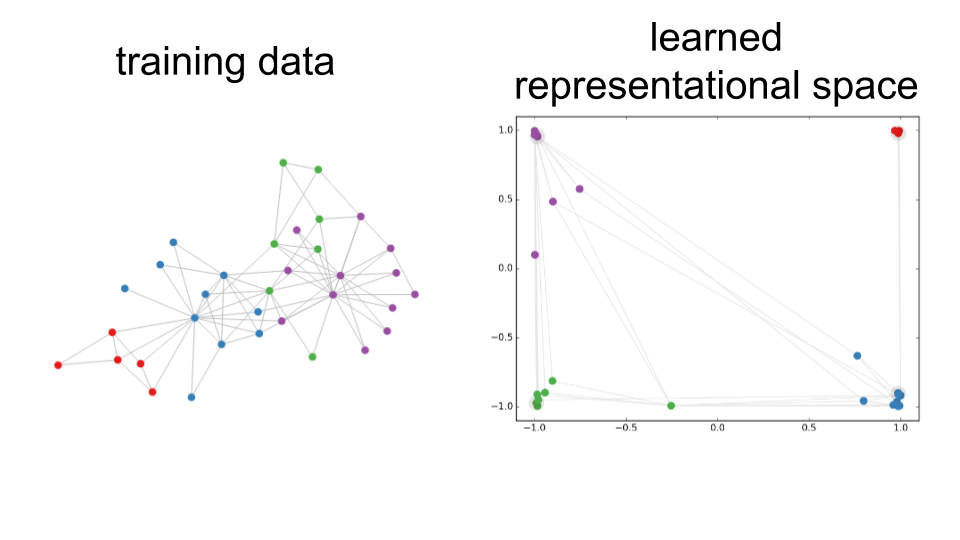
\includegraphics[scale=.4]{figures/kipf2016semi.png}
    \caption{Example of a graph embedding spaced learned by a Graph Convolutional Network (\cite{kipf2016semi}). Taken directly from \textcite{kipf2016semi}.}
\end{figure}

\textbf{\emph{Further Limitations of the Spatial Metaphor: Symmetry and the Triangle Inequality}:} Graph embedding spaces provide one preliminary avenue towards allowing spatial theories of similarity to leverage relational properties of a learning domain. However, there are other historical limitations with the spatial metaphor of similarity that are also present in graph embedding spaces: \emph{symmetry} and the \emph{triangle inequality problem}. Symmetry refers to the counterintuitive phenomenon where similarity judgments between 2 stimuli vary depending on presentation\footnote{which would be unusual if stimuli are represented as points in some vector space; the similarity between points A and B should be exactly the same as the similarity between points B and A} (\cite{tversky1977features,holyoak1983social,polk2002rating}; though see \cite{nosofsky1991stimulus}). For example, \textcite{tversky1977features} asked subjects to rate the similarity between a less and a more prominent country. \textcite{tversky1977features} found that subjects gave higher similarity ratings when the less prominent country was presented first\footnote{It is worth noting that many demonstrations of asymmetry utilize this type of sequential presentation (\cite{tversky1977features,polk2002rating}).}. This demonstration and others (\cite{holyoak1983social,polk2002rating}) highlight a clear symmetry violation in similarity ratings that deviates from a purely spatial interpretation of similarity perception\footnote{Interestingly, \textcite{polk2002rating} also found asymmetries between the number of processing cycles needed for a recurrent neural network to shift from one stimulus representation to another, which (a) might suggest an important role of recurrent computation in similarity perception, and (b) arguably lends support for \emph{transformational} theories of similarity (\cite{wiener1980analysis,imai1977pattern}).}.

The second limitation was raised by \textcite{tversky1982similarity}, who found conditions where human similarity perception violates a fundamental assumption of geometric spaces. More specifically, a geometric representational space requires that the distance between points \(A\) and \(C\) must always be less than the distance between points \(A\) and \(B\) plus the distance between \(B\) and \(C\); referred to as the \emph{triangle inequality} (\(dist(A,B) + dist(B,C) > dist(A,C)\); see figure \ref{fig:tversky}.a). \textcite{tversky1977features} provides an interesting set-theoretical alternative that doesn't make the same geometric assumptions of spatial similarity models. \textcite{tversky1977features}'s \emph{featural model} suggests that the similarity between 2 stimuli \(i\) and \(j\) reflects 3 important components: (1) shared features between the stimuli, (2) exclusive features of \(i\), and (3) exclusive features of \(j\) (see figure \ref{fig:tversky}.b; \textcite{tversky1977features,}); given by the equation:

$$ similarity(i,j) = \theta f(i \cap j) - \alpha f(i - j) - \beta f(i - j) $$ 

where \(\theta,\alpha,\beta\) are weights on some function \(f\). In \textcite{tversky1977features}'s model, there are no inherent assumptions requiring similarity ratings to follow the normal axioms of geometry (e.g., symmetry, the triangle inequality). Interestingly (and of relevance to this paper), \textcite{tversky1977features}'s featural model can be reformulated in the language of network science. For example, if stimuli and featural attributes are represented as connected nodes, than \textcite{tversky1977features}'s featural model can be framed as a computation on the resulting bipartite\footnote{\href{https://en.wikipedia.org/wiki/Bipartite_graph}{wikipedia's description of bipartite graphs}} graph. If we remove the weights and functions that transform each of the 3 components in \textcite{tversky1977features}'s model\footnote{which may arguably be too drastic of a change to the theory to make this exercise meaningful}, then the resulting similarity function can be described as the number of shared neighbors minus the number of distinct neighbors. 

\begin{figure}[h]
    \centering
    \label{fig:tversky}
    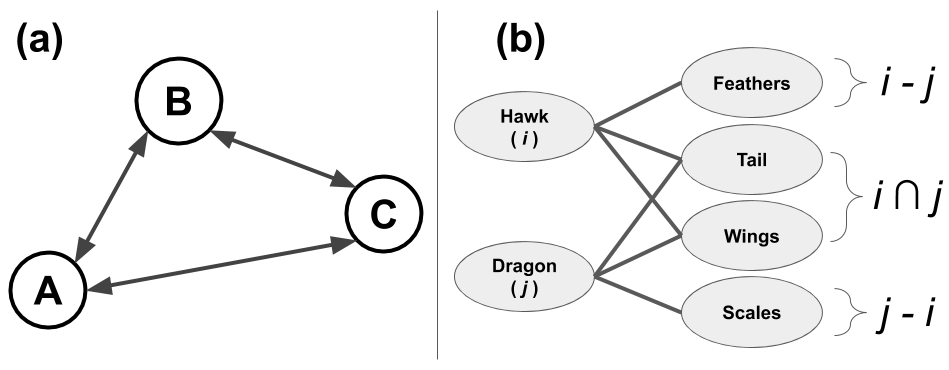
\includegraphics[scale=.4]{figures/tversky.png}
    \caption{\textbf{(a)} 3 stimuli plotted in geometric space. \textbf{(b)} \textcite{tversky1977features}'s featural model of the similarity between two items \(i\) and \(j\), visualized as a bipartite graph. }
\end{figure}

It's an open question whether there are benefits to framing \textcite{tversky1977features}'s feature model through the lens of network science beyond an appeal to Occam's razor. However, \emph{shared features} in a graph corresponds with another network science metric that has had notable consideration in the semantic similarity literature: path distance between two nodes (\cite{collins1975spreading,rada1989development,lee1993information,kenett2017semantic}). For example, \textcite{rada1989development} suggested that the average shortest path length between two nodes could accurately predict human semantic judgments. Additionally, \textcite{kenett2017semantic} found that path length predicted reaction times in discrete semantic relatedness judgments. These results, as well as the empirical success of \textcite{tversky1977features}'s featural model (\cite{tversky1982similarity}), leave open the possibility that network statistics might underlie various phenomena in the similarity perception literature\footnote{However, the spatial versus featural debate seems to have been reignited by the finding that distributional semantic models (which closely resemble the spatial metaphor of similarity) are also predictive of similarity judgments (\cite{bhatia2019distributed,gunther2016latent}; though see \cite{de2016predicting}), leaving this issue unresolved in the present literature.}.

\textbf{\emph{Subsection Conclusion}:} The concept of similarity has received over a century of attention from psychologists (\cite{james1890principles,attneave1950dimensions,tversky1977features,goldstone2012similarity}), but has been notoriously difficult to resolve. Similarity appears to be multifaceted, evident by the empirical success of many distinct theoretical camps (\cite{shepard1987toward,nosofsky1994comparing,tversky1977features,goldstone1991relational}). There may be key differences in the nuances of particular experimental preparations that predict when one theoretical model of similarity will succeed over another. For example, TACL experiments typically utilize isolated stimuli that collectively vary on a restricted set of shared features\footnote{e.g., size, shading, color} (\cite{kurtz2015human,nosofsky1994comparing}). The success of the spatial metaphor in this domain might be contingent on the typical lack of disjunctive features and relational statistics that would otherwise influence similarity perception\footnote{i.e., the second and third component of \textcite{tversky1977features}'s featural model reduce to zero}. Additionally, violations of the spatial metaphor are typically observed via sequential presentation of stimuli (as opposed to pairwise comparison), and typically use relatively complex, conceptual stimuli (\cite{tversky1977features,holyoak1983social})\footnote{But not in \textcite{polk2002rating}, who used color patches (which is arguably closer to stimuli used in a standard TACL experiment)}. The apparent inconsistencies in the spatial metaphor might also reflect the type of similarity space that theorists commonly invoke\footnote{\textcite{jakel2008similarity} suggest that Hilbert spaces might be better suited to serve the spatial metaphor of similarity} (e.g., city-block, euclidean). Beyond differences in methodological preparations, network science and graph statistics may also help explain similarity perception in the attribute category learning and relational similarity literature as well. 

% - - - - - - - - - - - - - - - - - - - - - 

\section{Graphs, Cognition, and Directions in Graph Learning Research}
    
Graph theory and network science might be useful in explaining many empirical observations in the category learning literature, such as category hierarchies (\cite{mervis1981categorization}), exemplar and prototype effects (\cite{danks2014unifying}), attention and unidimensional bias, and similarity perception. As discussed earlier in this paper, graphs have also been implicated language (\cite{vitevitch2008can,chan2009influence,chan2010network,vitevitch2012complex}), motor sequences (\cite{kahn2018network}), and event segmentation (\cite{karuza2017process,karuza2019human}). The next section will briefly highlight other domains in which graph theory and network science have been (and could be) invoked in explanatory models of cognition. Then, recent computational approaches to graph learning will be discussed.

\subsection{Graphs and Cognition}

\textbf{\emph{Causal Cognition}:} The ability for humans to recognize causal relationships between objects and events in their environment has been suggested as a hallmark of human cognition (\cite{penn2008darwin}). Internal mental or conceptual models are often invoked as the mediating construct of our causal cognitive abilities (\cite{murphy1985role,carey1985conceptual,springer1989development,barrett1993theory}). While the notion of a mental model is somewhat flexible\footnote{and arguably difficult to falsify}, many researchers have suggested that our causal understanding of the world is grounding in probabilistic graphical models (\cite{danks2014unifying,griffiths2010probabilistic,holyoak2011causal}). Probabilistic graphical models (or, Bayesian networks) are directed, acyclic\footnote{Acyclic refers to the constraint that no child node can be connected to its parent (i.e., no cycles); which arguably prevents circular reasoning} graphs (DAG) that represent objects or events as nodes and causal relationships as one-directional, weighted edges. Many theoretical explanations of causal cognition posit that the goal of the learner is to estimate useful parameters that best describe a graphical model of the learner's environment (\cite{danks2014unifying}). 

\begin{figure}[h]
    \centering
    \label{fig:bayesianNetwork}
    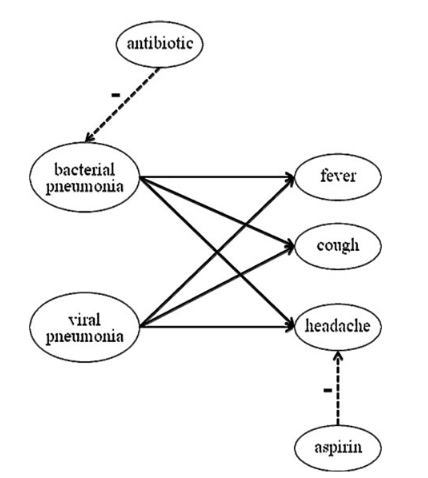
\includegraphics[scale=.4]{figures/bayesianNetwork.png}
    \caption{Example of a Bayesian network describing the causal connection between pathogens and experienced symptoms (taken directly from \cite{holyoak2011causal})}
\end{figure}

Unlike connectionist networks, probabilistic graphical models require an explicitly defined modular structure prior to parameter estimation\footnote{which researchers have argued makes Bayesian networks considerably more interpretable than connectionist networks (\cite{griffiths2010probabilistic})} (\cite{griffiths2010probabilistic}). However, because the latent structure of probabilistic graphical models are typically specified by the experimenter (\cite{mcclelland2010letting}), there is a large explanatory gap in how information from a noisy perceptual experience is mapped onto the relevant elements of a graphical representation (i.e., the binding problem). In contrast, connectionist networks excel at learning complex mappings between raw perceptual data and some desired behavior (\cite{lecun2015deep,he2015delving}). Interestingly, probabilistic graphical models can be fluidly integrated with connectionist algorithms to map real-world, complex perceptual data onto the latent variables of a graphical model using variational inference techniques (\cite{johnson2016composing}), potentially bridging the gap between emergent (\cite{mcclelland2010letting}) and structured (\cite{griffiths2010probabilistic}) approaches to explaining semantic and causal cognition\footnote{which may reduce down to a question of where certain aspects of cognition reside on a scale ranging from completely distributed to completely modular (given that both connectionist and Bayesian networks are both different types of graphs; \cite{griffiths2010probabilistic})}. It may also explain how simple, associative learning mechanisms can produce a representation of conditional relationships between objects and events.


\textbf{\emph{Graphs and Analogical Reasoning}:} Analogical reasoning is also considered to be a hallmark of human intelligence (\cite{penn2008darwin}), its importance ranging from normal cognitive behavior to systematic scientific discovery (\cite{gentner1997reasoning,gust2008analogical,black1966models}). A common theme in many theories of analogical reasoning is the invocation of structured representations that explicitly isolate object relations from object features (\cite{gentner1983structure,forbus2017extending,hummel1997distributed,doumas2008theory,larkey2003cab})\footnote{This isolation is supported by evidence of a dissociation between relational and featural similarity judgments of human subjects (\cite{goldstone1991relational})}. In her seminal paper on analogical reasoning, \textcite{gentner1983structure} describes knowledge representation as a propositional network: \emph{relations} and \emph{attributes} serve as predicates that leverage \emph{features}, \emph{objects}, and \emph{relations}\footnote{\textcite{gentner1983structure} defines higher-order relations as relational predicates that take other relations as arguments} as arguments. This use of predicate calculus\footnote{See \textcite{rensink2004representing} for a demonstration on how predicate calculus (or, first-order logic) can be represented as a graph} to describe structured representations is a common element of many distinct computational models of analogical reasoning (\cite{forbus2017extending,hummel1997distributed,doumas2008theory,larkey2003cab}). In contrast with the approach offered by \textcite{gentner1983structure}, \textcite{kemp2004discovering} suggest that relational systems themselves can be represented as graphs where objects/entities are represented by nodes and relations are represented by edges. \textcite{kemp2010probabilistic} demonstrate how probabilistic models can leverage this representational style for theory discovery. Both of these approaches leverage networks as the fundamental data structure of knowledge representation, suggesting that network science may play a key role in explaining many hallmark characteristics of human intelligence.
% ^ this whole section is really bad


\textbf{\emph{Object Perception and Scene Grammars}:} Graphical structured representations have a history of being invoked in theories of object perception and scene understanding (\cite{pylyshyn1973mind,biederman1987recognition,hummel1992dynamic}). For example, \textcite{pylyshyn1973mind} argued that mental imagery of objects and scenes were mediated primarily by propositional representations\footnote{Recall the close connection between propositional logic and graphs (\cite{rensink2004representing})}, leveraging the symbolic, recursive mechanisms that (Pylyshyn argues) mediate language (\cite{chomsky1965aspects}). \textcite{biederman1987recognition}'s very influential \emph{Recognition-by-components} theory suggests that wholistic object perception is grounded in a relational hierarchy of simple geometric components (or, \emph{geons}). \textcite{han2008bottom} utilize hierarchical, graphical representations of objects in scenes (which they refer to as \emph{attribute grammars}) for parsing simple shapes from natural images. The theoretical notion that visual understanding leverages the same fundamental representational structure as language, causal reasoning, and analogy is particularly attractive: it allows various aspects of cognition from a variety of learning domains to be explained by a relatively restricted set of computational principles (\cite{griffiths2010probabilistic})\footnote{\textcite{griffiths2010probabilistic}, who originally suggested graphical models as the common representational structure of vision, language, and causal reasoning in 2010, also argued that Bayesian probabilistic networks were a good candidate for this unification endeavor}.

While a graphical explanation of object and scene understanding is compelling, it faces the same fundamental problem of mapping objects from a continuous perceptual stream into their respective roles in structured representation. Typically, this task is handled using hand-coded representations generated by the experimenter, which \textcite{chalmers1992high} argue leaves many important questions unanswered. Both probabilistic graphical models and connectionist models have historically suffered from this limitation (\cite{torralba2011learning,hinton1981shape,hummel2004solution}). However, deep learning algorithms might provide a tentative solution. Deep learning models are particularly useful for learning statistically useful visual features that can be leveraged as constituent elements in Bayesian probabilistic models (\cite{torralba2011learning,johnson2016composing}). \textcite{santoro2017simple} used features from a convolutional network (CNN) as objects in a relational learning model that achieved relatively high performance on the CLEVR\footnote{which tasks a model with answering questions about the spatial relations between simple geometric objects} dataset (\cite{johnson2017clevr}). Given that deep learning is undergoing preliminary success as an explanatory model of human visual perception (\cite{peterson2016adapting,long2018mid,khaligh2014deep}), deep learning models might be the tentative, psychologically-plausible\footnote{relatively speaking} bridge between sensory perception and structured representations of objects and scenes (though see \cite{baker2018deep}, \cite{baker2018illusory}, and \cite{erdogan20163d} for key explanatory limitations of deep learning models in their present form)\footnote{However, note that these demonstrations do not consider the recent work leveraging deep networks for structured representations (discussed in this section), leaving open the question of the explanatory value of deep learning in cognitive science}.

% - - - - - - - - - - - - - - - - - - - - - 

\subsection{Methodological Paradigms for Studying Graph Learning in Humans}

How humans behave in graph structured learning domains is an emerging field of research, already garnishing some promising results (\cite{lynn2019graph,kahn2018network,karuza2017process,wu2020inference}). However, the number of available paradigms is somewhat limited. Much of the work suggesting human sensitivity to network structure relies on the sequential presentation of stimuli in isolation, where the structural relations are defined by the transition probability from one stimulus to another (\cite{kahn2018network,karuza2017process,zurn2020network}). While work on transition graphs are a promising avenue for integrating network science and human cognition, it arguably embodies a particular type of homogeneous relation that might motivate distinct learning strategies relative to other types of relations (such as semantic or spatial)\footnote{Additionally, the relations present in semantic networks are often very heterogeneous}. 

Another interesting question in the graph learning literature is the impact of manipulating the statistical relationships between stimulus features in addition to network topology. Early steps in answering this question have recently been taken by \textcite{wu2020inference}. In one experiment, \textcite{wu2020inference} had subjects view an entire graph where each node was defined by a single feature (number of passengers at a train station). Subjects were asked to guess the feature value of an unlabeled node, ideally using information about other connected nodes in the graph to guide their judgments. Importantly, \textcite{wu2020inference} found that subjects were able to improve their judgments about the functional relationship between node features as the task progressed. In contrast with work using transition probabilities, subjects in \textcite{wu2020inference}'s experiment were shown the entire graph structure on each trial. The use of entire graphs as stimulus presentation provides an interesting addition to the presently limited number of paradigms where subjects are explicitly given local information alone\footnote{In a sense, these two paradigms elicit graphical inference in opposite directions (global to local versus local to global)}.

\begin{figure}[h]
    \centering
    \label{fig:wu2020task}
    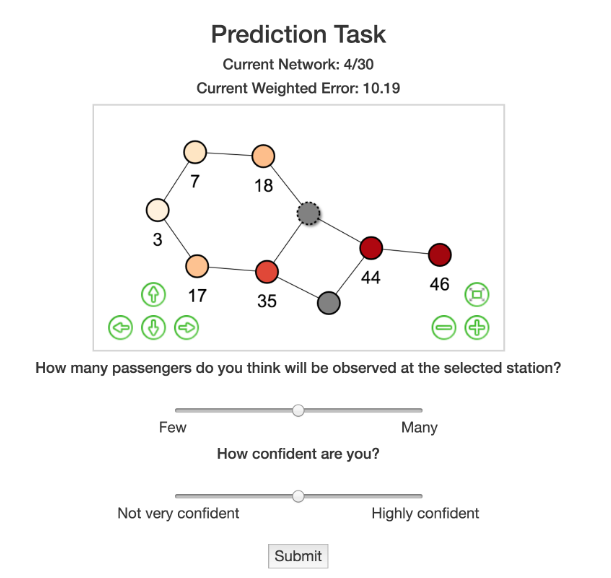
\includegraphics[scale=.4]{figures/wu2020task.png}
    \caption{Example of the preparation used in \textcite{wu2020inference}'s graph learning experiment (taken directly from \cite{wu2020inference})}
\end{figure}

Though research in network science seems to be progressing rapidly, there are still many unanswered questions regarding how network structure influences human cognition, particularly in the domain of category learning. Given evidence that English-words and semantic concepts embody a network structure (\cite{vitevitch2008can,steyvers2005large}), and the potential implication of network structure in perceptual segmentation (\cite{saffran1996statistical}), it would be interesting to investigate whether humans leverage network structure during the unsupervised formation of categorical knowledge. This might be addressable using a modification to the traditional paradigm for classification learning. Rather than in isolation, stimuli could be presented in pairs and subjects could be tasked with learning about the presence of a relationship between the co-presented stimuli (instead of a category label). Whether subjects leverage network structure for unsupervised categorization could be addressed using a free sort task after learning (\cite{medin1987family}).

% - - - - - - - - - - - - - - - - - - - - - 
\subsection{Connectionist Approaches to Graph Learning}

Learning and inference of graph structured data has become an increasingly popular topic in the machine learning literature (\cite{bronstein2017geometric}). Connectionist models have achieved relative success at tackling very difficult graph learning problems (\cite{kipf2016semi,graves2016hybrid,schlichtkrull2018modeling}). Given connectionism's rich history in psychology (\cite{mcclelland1987parallel,mcclelland2010letting,hummel2004solution})\footnote{Prior to the recent interest in geometric deep learning, there have been many other attempts to integrate structured representations into connectionist models (\cite{pollack1990recursive,smolensky1990tensor})}, it might be interesting to explore whether geometric deep learning algorithms have any predictive value as models of human reasoning in graph structured domains. At the very least, they suggest that the associative, error-driven mechanisms of traditional connectionist models are a powerful tool for learning and inference on structured and unstructured data. Though as stated earlier, there are many distinct implementations of geometric deep learning algorithms, some of which may provide more promising avenues for cognitive scientists than others. 

In particular, many variants of geometric deep learning algorithms rely on an aggregation step that collapses over nodes in a neighborhood during training (\cite{wu2020comprehensive}). This aggregation step places considerable constraints on the types of local neighborhood structures that geometric deep learning algorithms can differentiate (\cite{xu2018powerful}), and prevents models from capitalizing on intra-neighborhood variability. This limitation is circumvented by \textcite{velivckovic2017graph}, who leveraged the attention mechanisms that have seen recent success in natural language processing (using a model they call \emph{Graph Attention Networks}, or GATs). GATs are a particularly appealing avenue for modeling human reasoning, given that they utilize similar computational mechanisms for both relational reasoning and language comprehension. Another recent approach in applying connectionist learning algorithms to graph structured learning domains comes from work on memory-augmented networks (\cite{graves2016hybrid}). Using a combination of memory and attention, \textcite{graves2016hybrid} found that a recurrent network trained on randomly generated graphs could efficiently navigate other graph structured learning domains (such as graph representations of subway tunnels or family trees). Interestingly, \textcite{graves2016hybrid} suggest preliminary parallels between their model and hippocampus-mediated human memory.

\begin{figure}[h]
    \centering
    \label{fig:DNC}
    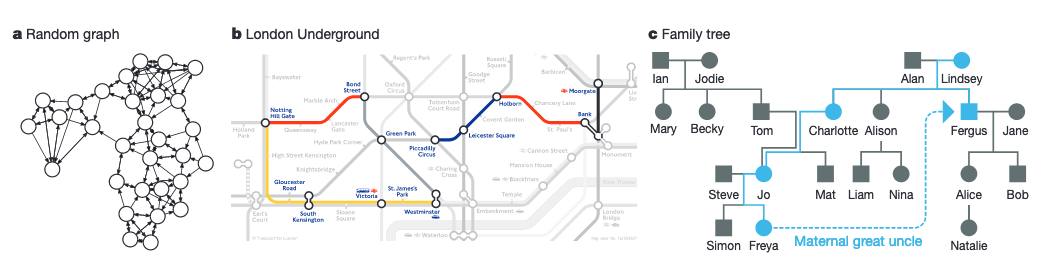
\includegraphics[scale=.4]{figures/DNC.png}
    \caption{Example of the learning domains that \textcite{graves2016hybrid}'s \emph{differentiable neural computer} was able to (arguably) generalize between (taken directly from \cite{graves2016hybrid})}
\end{figure}

% - - - - - - - - - - - - - - - - - - - - - 

\section{Conclusions}

A number of demonstrations have provided preliminary evidence that humans are sensitive to the network characteristics of graph structured learning domains (\cite{lynn2019graph,karuza2019human,kahn2018network,wu2020inference}). Graphs have also been implicated as a representational structure across many different literatures\footnote{either as large scale relational systems or as predicate networks} (\cite{abbott2012human,vitevitch2008can,gentner1983structure,griffiths2010probabilistic}). Additionally, many puzzling phenomena in the category learning literature seem reasonably intuitive when viewed through the lens of network science. The widespread use of network structures in psychological theories and the recent application of graphs for tackling very difficult cognitive challenges (\cite{wu2020comprehensive,hamrick2018relational,han2008bottom,graves2016hybrid}) suggest that graphs might be a fundamentally important, cross-domain data structure for cognitive representations.




% - - - - - - - - - - - - - - - - - - - - - 
% - - - - - - - - - - - - - - - - - - - - - 


% % % % % % % % % %
%
%   REFERENCES
%
% % % % % % % % % %

\pagebreak
\pagestyle{empty}
\renewcommand\bibname{References}
\printbibliography

% - - - - - - - - - - - - - - - - - - - - - 
% - - - - - - - - - - - - - - - - - - - - - 


% % % % % % % % % %
%
%   APPENDIX
%
% % % % % % % % % %
\pagebreak
\appendix
\appendixpage
\addappheadtotoc

\section{Details of Network Generation Examples}

\textbf{\textcite{steyvers2005large}'s Growing Network Model:} To examine the impact of density on the properties of large scale networks, the network generation algorithm from \textcite{steyvers2005large} was used to generate a large set of 24 networks of node size 200. The algorithm starts off by generating a fully connected set of \(M\) nodes. After initialization, a new node is added to the network. The new node is connected to \(M\) neighbors of an already existing node \(i\). The existing node \(i\) is selected from a distribution:

$$ P_{i} = \frac{k_i}{\sum{k_n}} $$

where \(k_i\) is the degree of a random node and \(\sum{k_n}\) is the sum of the degrees of all nodes in the network. The \(M\) connections between the new node and the neighborhood of node \(i\) are sampled uniformly. This repeats until the algorithm reaches the desired network size.

% - - - - - - - - - - - - - - - - - - - - - 
% - - - - - - - - - - - - - - - - - - - - - 

\end{document}
